\chapter{Felhasználói dokumentáció}
\label{ch:user}

A következő fejezetben bemutatom, hogy az álltalam fejlesztett kiegészítőt, illetve a kiegészített szoftvereket hogyan kell telepíteni, beüzemelni, illetve használni, képekkel illusztrálva.

\section{Rendszerkövetelmények}

\begin{itemize}
    \item Hardver
    \begin{itemize}
        \item 2 GHz vagy nagyobb órajelű processzor
        \item 2 GB RAM memória
        \item 1 GB lemezterület a RefactorErl, Visual Studio Code, Erlang LS, illetve a bővítmény számára (forráskódok betöltéséhez további tárhely és memória szükséges)
    \end{itemize}
    \item Szoftver
    \begin{itemize}
        \item mac OS El Capitan, Windows 10 vagy Linux operációs rendszer
        \item Telepített RefactorErl elemző eszköz
        \item GraphViz 2.38 (a függőségi gráf rajzolásához)
        \item Erlang/OTP 22 vagy újabb
        \item Visual Studio Code 1.67.0 (Universal)
        \item GCC 4.7.2 vagy újabb fordítóprogram
    \end{itemize}
\end{itemize}

\section{Telepítés}

A fejlesztés mac OS operációs rendszeren történt, így a legtöbb helyen a telepítési útmutató részlétesebb leírást tartalmaz ezen operációs rendszerhez. Azonban a mind az újonnan fejlesztett komponensek (Visualiser kiegészítő) és a RefactorErl, illetve az Erlang LS működik Windows és Linux operációs rendszerek alatt is.

\subsection{Erlang/OTP telepítése}

Mind a RefactorErl futtatásához, mind az Erlang LS futtatasához szükségünk van az Erlang virtuális gép telepítéséhez. Ezt macOS operációs rendszer legegyszerűbben a Homebrew \cite{homebrew} nevű csomagkezelővel tehetjük meg az alábbi parancs kiadásával:

\noindent \lstinline{brew install erlang}

Linux és Windows rendszerekhez az Erlang honlapjáról \cite{erlangDownloads} tájékozódhatunk a telepítő parancsokról, illetve innen tölthetjük le a telepítő állományt is.

\subsection{GCC telepítése}
A GNU/GCC fordító szükséges az Erlang és a RefactorErl egyes komponenseinek fordításához, így telepítése szükséges. Ezt legegyszerűbben szintén az operációs rendszerünk csomagkezelőjével megtehetjük. Mac OS operációs rendszer alatt, itt is használhatjuk a Homebrew \cite{homebrew} csomagkezelőt, az alábbi paranccsal:
\noindent \lstinline{brew install gcc}

További információért keressük fel a GNU/GCC hivatlos oldalát. \cite{gnuGcc}.

\subsection{Graphviz telepítése}
A GraphViz telepítése opcionális, azonban a gráfok kirajzolásához szükséges. Ezt szintén legegyszerűbben az operációs rendszerünk csomagkezelőjével tehetjük meg. Amennyiben további információra van szükségünk, keressük fel a GraphViz oldalát \cite{graphviz}, ahol telepítő csomagok és parancsok is rendelkezésre állnak.
Mac OS operációs rendszer alatt, használhatjuk az alábbi parancsot:
\noindent \lstinline{brew install graphviz}

\subsection{Yaws webszerver telepítése}
A YAWS\footnote{Yet Anothet Web Server} forráskódja letölthető és telepíthető a GitHub oldalukról \cite{yawsGithub}, ahol a \lstinline{README} fájlban megtalálhatóak a telepítéshez szükséges utasítások.

Mac OS operációs rendszer alatt használhatjuk a Homebrew csomagkezelőt \cite{homebrew} is, az alábbi parancs kiadásával:
\noindent \lstinline{brew install yaws}

\subsection{RefactorErl telepítése}
A RefactorErl hivatalos kiadása letölthető az eszköz honlapjáról \cite{refactorErlWebsite}, azonban a \textit{szakdolgozat készítésének időpontjában a publikus verzióban a szükséges modulok még nem elérhetőek, de a következő kiadásban jelen lesznek}. Természetesen a szükséges modulokat tartalmazó verzió megtalálható a szakdolgozat mellékleteként.

Telepítéshez csomagoljuk ki a RefactorErl forrását tartalmazó tömörített állományt, majd lépjünk be a gyökérkönyvtárába.

\noindent Telepítés Windowson: \lstinline{bin\referl -build tool -yaws_path path\to\yaws}
\noindent Telepítés Linuxon: \lstinline{bin/referl -build tool -yaws_path path/to/yaws}

Ahol a \lstinline{-yaws_path} kapcsoló utána a YAWS \lstinline{ebin} könyvtárának elérhetőségét kell megadni. 

\subsection{Visual Studio Code telepítése}
A Visual Studio Code egy cross-platform\footnote{többféle rendszeren képes futni} fejlesztői környezet, ami igen gazdag fejlesztői interfésszel rendelkezik, ami lehetővé tette ezt a fejlesztést is. Megfelelő operációs rendszer kiválasztása után letölthető a termék honlapjáról \cite{vscodeWebsite}.

\subsection{RefactorErl Visualiser telepítése}
A Visualiser bővítmény letölthető a bővítmény GitHub oldaláról: \url{https://github.com/robertfiko/refactorerl-visualiser}. Ezután a \lstinline{make visualiser} paranccsal fordítható és telepíthető, de javasolt inkább a mellékelt állományok között is megtalálható a \lstinline{.vsix} kiterjesztésű telepítő fájl használata. 

A telepítéshez menjünk a bővítmények menübe a Visual Studio Code-on belül. Ezt a bal oldali oldalmenüben találjuk meg. Majd a megjelenő oldalsáv jobb felső sarkából a három pontra (\lstinline{...}) kattintva válasszuk az "\textit{Install from VSIX ...}" opciót, majd a felugró ablakban keressük ki a VSIX fájlt. (lásd: \ref{fig:vsix_install} ábrán)

\textit{Megjegyzés: amennyiben rendelkezünk GNU/MAKE-el abban az esetben a \lstinline{make refels} paranccsal az Erlang LS bővített verziója is telepíthető a Git tárolójából, de nem ezt az eljárás módot fogjuk követni.}


\begin{figure}[H]
  \centering
  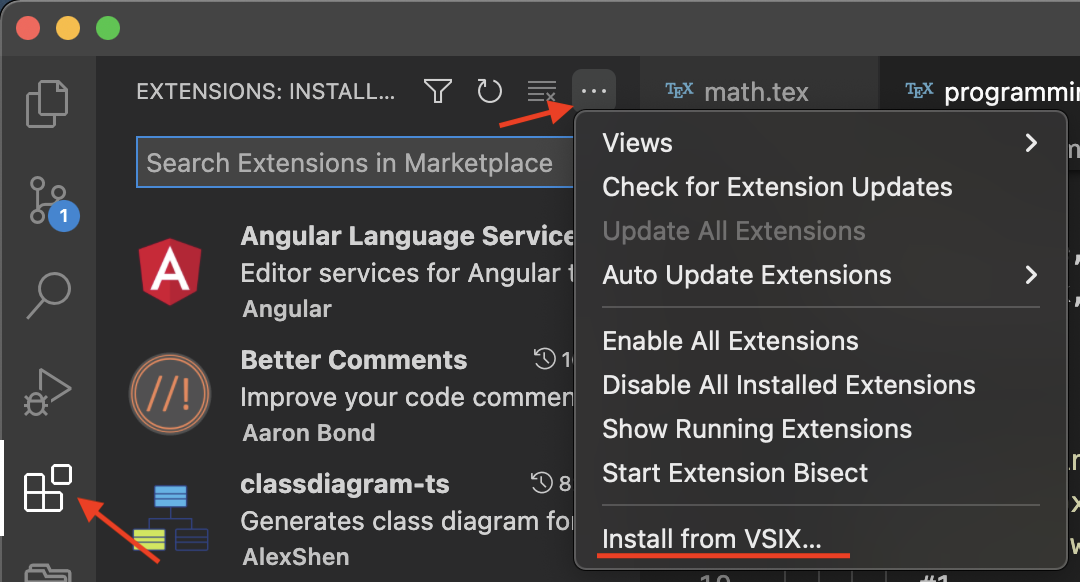
\includegraphics[width=\linewidth]{images/vsix_install.png}
  \caption{Telepítés \lstinline{.vsix} fájlból}
  \label{fig:vsix_install}
\end{figure}

\subsection{Erlang LS bővített változatának telepítése}
Az Erlang Language Server \textit{eredeti verziója} megtekinthető a GitHub tárolójában \footnote{\url{https://github.com/erlang-ls/erlang_ls}}, illetve letölthető a Visual Studio Code Marketplace\footnote{\url{https://marketplace.visualstudio.com/items?itemName=erlang-ls.erlang-ls}}-ről .

A bővített verzió forráskódja megtalálható a dolgozat csatolmányai között, s az ebből előálló \lstinline{.vsix} fájl is. Ezt a már korábban a \ref{fig:vsix_install} ábrán mutatott módon telepíthetjük.

\section{Erlang LS használata}
\subsection{Első elindításkor szükséges beállítási lehetőségek} \label{ELSfirstStart}
Az első elidulás előtt az Erlang LS konfigurációs \cite{erlangLsConfig} fájljában néhány módosítást kell végeznünk, hogy az megfelelően illeszkedjen a RefactorErlhez. A konfigurációs fájl YAML formátumot követ. 
A diagnosztikák futtatásához vegyük fel a \lstinline{refactorerl} elemet az engedélyezettek közé. 

\lstset{caption={RefactorErl diagnosztikák engedélyezése Erlang LS-ben}, label=src:yaml}
\begin{lstlisting}
diagnostics:
  enabled:
    - refactorerl
\end{lstlisting}

\textit{Erlang node-nak nevezzük az Erlang virtuális gép egy példányát. Gyakran csak egszerűen node-ként fogok rá hivatkozni. A RefactorErl node alatt pedig azt az Erlang virtuálsi gép példányt értjük, amin az eszköz fut.}

Ezzel a beállítással az Erlang LS már futtatni fogja a diagnosztikákat, azonban alapértelmezetten egyetlen diagnosztikai sem fog futni, ezeket manuális allíthatjuk be. Ehhez vegyünk fel egy \lstinline{refactorerl} kulcsot a fájl gyökerébe. Ez alá két \textit{alkulcs} kerülhet:
\begin{itemize}
    \item \lstinline{node}: ide annak az Erlang node-nak a nevét kell megadni szöveges karakterláncként, ahol a RefactorErl fut. 
    \item \lstinline{diagnostics}: azon diagnosztikák azonosítói, amelyeket futtatni szeretnék listaként (felsoroláskén) megadva. A dignosztikák azonosítói szintén szöveges karakterláncok.
\end{itemize}

Példa egy ilyen konfigurációs fájl részletre:

\lstset{caption={RefactorErl konfigurációs példa Erlang LS-ben}, label=src:yaml}
\begin{lstlisting}
diagnostics:
  enabled:
    ...
    - refactorerl

...

refactorerl:
  node: "nodeName@hostName" 		
  diagnostics:
    - "unused_macros"			
    - "unsecure_os_call"
\end{lstlisting}

Az alábbi diagnosztikákból tudunk válogatni jelenleg:


\begin{longtable}{|m{0.4\textwidth}|m{0.5\textwidth}|}
 \hline
 Lekérdezés neve & Lekérdezés rövid ismertetése \\ [0.5ex] 
 \hline\hline
 \verb|unused_macro| & Nem használt makró definíciók megjelenítése \\ \hline
 \verb|unsecure_calls| & Az összes lehetséges támadási forma megjelenítése \\ \hline
 \verb|unsecure_interoperability| & Az együttműködési képességből fakadó sebezhetőségek azonosítása. \\ \hline
 \verb|unsecure_concurrency| & A konkurens programozásból eredő hibalehetőségek feltérképezése. \\ \hline
 \verb|unsecure_os_call| & Az ismeretlen helyről származó paraméterekkel meghívott OS szintű utasítások ellenőrzése. \\ \hline
 \verb|unsecure_port_creation| & A portok létrehozásával kapcsolatos sebezhetőségek megjelenítése. \\ \hline
 \verb|unsecure_file_operation| & Az ismeretlen bemenettel meghívott fájlkezeléssel kapcsolatos műveletek megjelenítése. \\ \hline
 \verb|unstable_call| & Az atomok dinamikus létrehozásával kapcsolatos függvények feltérképezése. \\ \hline
 \verb|nif_calls| & A NIF függvények használatából fakadó sebezhetőségek ellenőrzése. \\ \hline
 \verb|unsecure_port_drivers| & A dinamikusan betölthető könyvtárak használatából fakadó veszélyek azonosítása. \\ \hline
 \verb|decommissioned_crypto| & Az elavultnak számító kriptográfiai műveletek megjelenítése. \\ \hline
 \verb|unsecure_compile_operations| & Az ismeretlen helyről származó programkód fordításának és betöltésének ellenőrzése. \\ \hline
 \verb|unsecure_process_linkage| & A folyamatok nem megfelelő összekapcsolásából adódó sebezhetőségek megjelenítése. \\ \hline
 \verb|unsecure_prioritization| & A folyamatok prioritásának módosításából fakadó veszélyek ellenőrzése. \\ \hline
 \verb|unsecure_ets_traversal| & Az ETS tábla rögzítés nélküli bejárásának ellenőrzésére szolgáló megjelenítése. \\ \hline
 \verb|unsafe_network| & A hálózati rendszermaggal kapcsolatos műveletek feltérképezése. \\ \hline
 \verb|unsecure_xml_usage| & Az ismeretlen helyről származó xml paraméterek elemzésével kapcsolatos függvények azonosítása. \\ \hline
 \verb|unsecure_communication| & Az elosztott hálózat szereplői között zajló kommunikációs beállítások ellenőrzése. \\ [1ex] 
 \hline
\caption{Elérhető diagnosztikai azonosítók listája.}
\label{table:1}
\end{longtable}

\subsection{A RefactorErl konfigurálása} \label{referlConfig}

Ahhoz megfelelő válaszidővel és teljesítménnyel tudjunk dolgozni a Erlang LS-ben RefactorErl-el vagy a Visualiser bővítménnyel érdemes már egy konfigurált adatbázist készíteni, hogy az elemzések zömét mér elvégezze az eszköz, s használat közben csak esetleges szinkronizációkat kelljen végezni, amikor csak a változtatásokat kell leelemezni. A RefactorErl használatának részletei megtekinthetőek az eszköz Wiki oldalán. \cite{referlWiki}

Az adatbázishoz az \lstinline{ri:add} függvény segítségével adhatunk fájlokat. Megadhatunk paraméterként egy fájlnevet karakterláncként, vagy úgynevezett atomként\footnote{Az Erlang nyelvben atomnak nevezünk egy olyan literált, aminek értéke megegyezik a nevével, amit egyfajta szövegkonstansnak is nevezhetünk.}. Ebben az esetben a lokális útvonal a jelenlegi könyvtár, amiben dolgozunk. Természetesen globális útvonalként is megadhatunk fájlokat. Amennyiben könyvátarat adunk meg, akkor az adott könyvtárat rekurzívan bejárva az összes fájl hozzá lesz adva. Néhány példa a használatra \cite{referlWikiFileManagement}:

\noindent \lstinline{cd(dir), ri:add(modname).}\\
\noindent \lstinline{ri:add('dir/modname').}\\
\noindent \lstinline{ ri:add("dir/modname.erl").}\\
\noindent \lstinline{ri:add("path_to_dir/dir").}\\

Ezen kívül az \lstinline{ri:ls().} paranccsal lekérhetjük a beolvasott fájlok listáját, az \lstinline{ri:reset().} segítségével pedig törölhetjük az adatbázist.


\subsection{Diagnosztikák használata}
Az Erlang LS a diagnosztikákat az adott szerkesztőben figyelmeztetésként jeleníti meg. Ugyan ez a funckionalitás \textbf{minden ELS-el kompatibilis szerkesztőben meg fog jelenni}, most a példák során a Visual Studio Code szerkesztőre fogunk fókuszálni. Miután a konforgurációs fájlban mindent beállítotunk (ld. \ref{ELSfirst} bekezdés) nincs más dolgunk, mint betölteni egy forráskódot és megtekinteni az eredményt.

\subsubsection{Példa: Nem használt makró definíciók}

Az alábbiakban a \lstinline{unused_macros} azonisítójú diagnosztikát fogjuk áttekinteni. Ehhez nézzük meg alábbi a forrást:

\lstset{caption={Nem használt makró definíciókkal eláttot szemléltető kód}, label=src:erlang}
\begin{lstlisting}[language={Erlang}]
-module(show).
-define(PRIME, 7).
-define(NOT_PRIME, 12).

show_prime() ->
    ?PRIME.
\end{lstlisting}

Itt láthatjuk, hogy a \lstinline{NOT_PRIME} makró nincs használatban. Ha megnézzük, milyen diagnosztikákat kaptunk a RefactorErltől, az Erlang LS-en keresztül akkor láthatjuk, hogy figyelmesztetés szintű diagnosztikát jelez nekünk.

\begin{figure}[H]
  \centering
  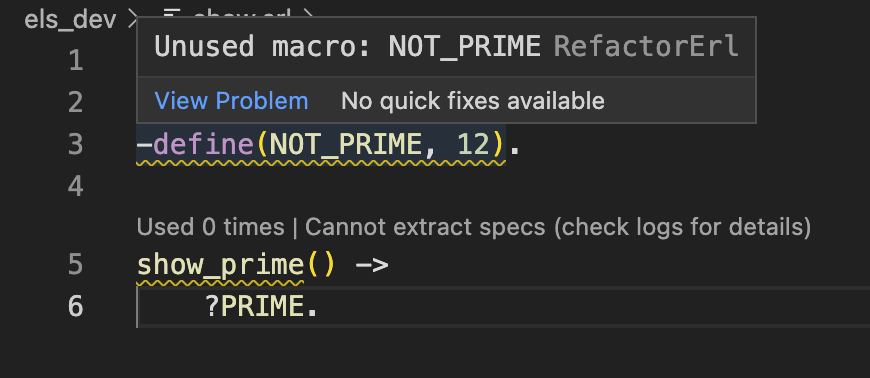
\includegraphics[width=0.7\linewidth]{images/undefined_macro.png}
  \caption{Nem használt makró diagnosztika Visual Studio Code-ban}
  \label{fig:unused_macro_vscode}
\end{figure}


\subsubsection{Példa: Nem biztonságos \lstinline{os} hívás diagnosztika}

\lstset{caption={Nem biztonságos \lstinline{os} hívást szemléltető kód}, label=src:erlang} 
\begin{lstlisting}[language={Erlang}] 
-module(show).
-export([safe_os_call/0, unsafe_os_call/1]).

safe_os_call() ->
    os:cmd("ls").

unsafe_os_call(A) ->
    os:cmd(A).
\end{lstlisting}

A fenti forrásban ötödik sorban lévő \lstinline{os:cmd} hívást nem tekintjük veszélyforrásnak, hiszen a fejlesztő maga paraméterezi fel. Azonban hetedik sorban kezdődő \lstinline{unsafe_os_call} definíciót sérülékenységi pontnak tekintjük, hiszen paramétere ismeretlen helyről származik \cite{refactorerlSecurity}.

Ennek megfelőlen a \ref{fig:unsafe_os_call_vscode} ábrán láthatjuk is, hogy a szerkesztő program figyelmeztetést is adott a szóbanforgó kódrészletre. 

\begin{figure}[H]
  \centering
  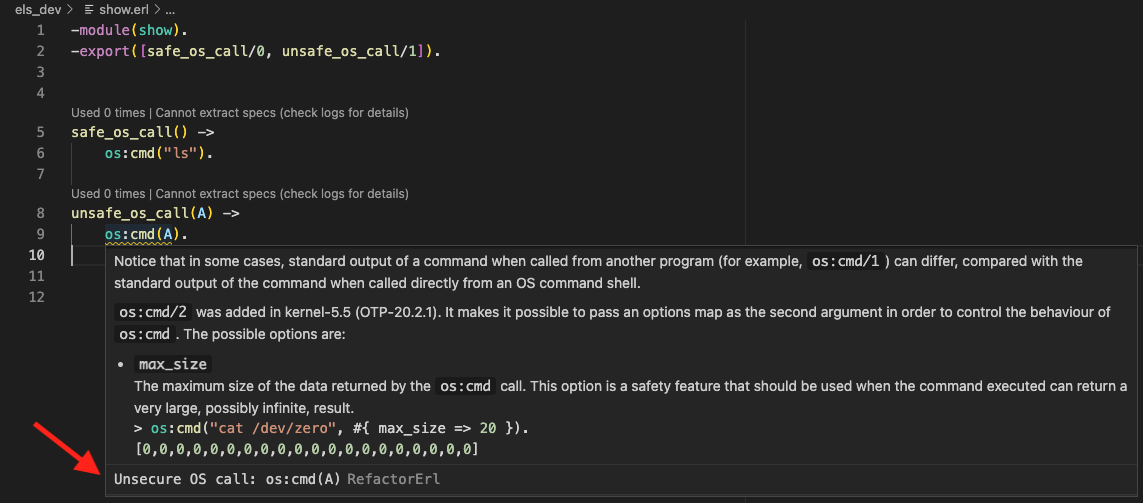
\includegraphics[width=\linewidth]{images/unsafe_os_with_safe_os.png}
  \caption{Nem biztonságos \lstinline{os} hívás diagnosztika Visual Studio Code-ban}
  \label{fig:unsafe_os_call_vscode}
\end{figure}

Ezen fejezetnek nem célja bemutatni az összes lehetséges diagnosztikát, csupán egy átfogó képet adni, azok használatáról. Továbbiakban az felhasználóra van bízva, hogy mely diagnosztikát szeretné használni. Az integrált diagnosztikák jelentős része Baranyai Brigitta TDK dolgozatából származik, ahol további részletekről is olvashatunk \cite{refactorerlSecurity}.


\subsection{Kódakció parancsok kiadása}

\textit{Egy változó Origin értékének vagy eredetének azt mondjuk, hogy melyek azok a lehetséges értékek, amelyek a kiírtékelés során belefolyhatnak.} \cite{macs10paper} \cite{cefp11paper} 

\textit{Egy változó Reach értékén azt értjük, hogy az adott változó értéke mely helyekre folyhat be, ahol az ki lesz értékelve.} \cite{macs10paper} \cite{cefp11paper} 

A kódakciók, avagy angolul \textit{Code Actions} a fejlesztői környezetben megjelenő gyors javítások, refaktorálások és tanácsok. Jelenleg inkább az első kettő megközelítés az elterjedt, ahogyan azt a Visual Stuido Code felhasználói útmutatója is írja. \cite{vscodeCodeActionUserGuide}. Ebben a dolgozatban ezen funkciót kissé kiterjesztve, kód értelmezési funkcionalitást kapott. Kódakcióként elérhetőek az alábbi funkciók:

\begin{itemize}
    \item Függőségi gráf lekérése adott függvényből vagy modulból kiindulva
    \item Változó Origin értékének lekérése
    \item Változó Reach értékének lekérése
    \item Függvény (dinamikus) hivatkozásainak lekérése
\end{itemize}


Ugyan a fent felsorolt funkcionalitások az Erlang LS felületéről indulnak, azonban sajnos a \textit{Language Server Protocol} limitációi miatt, ezen funkciók, lekérdezések megjelenítésére nincsen lehetőség \cite{microsoftLSp}. Ezen limitációk áthidalására készült a RefactorErl Visualiser bővítmény. A lekérdezések eredményének megjelenítéséről gráf rajzolása esetében \ref{sectionDepGraph} fejezetben, míg a Reach, Origin és függvények hivatkozás esetében a \ref{sectionVariable} fejezetben olvashatunk.

\begin{figure}[H]
  \centering
  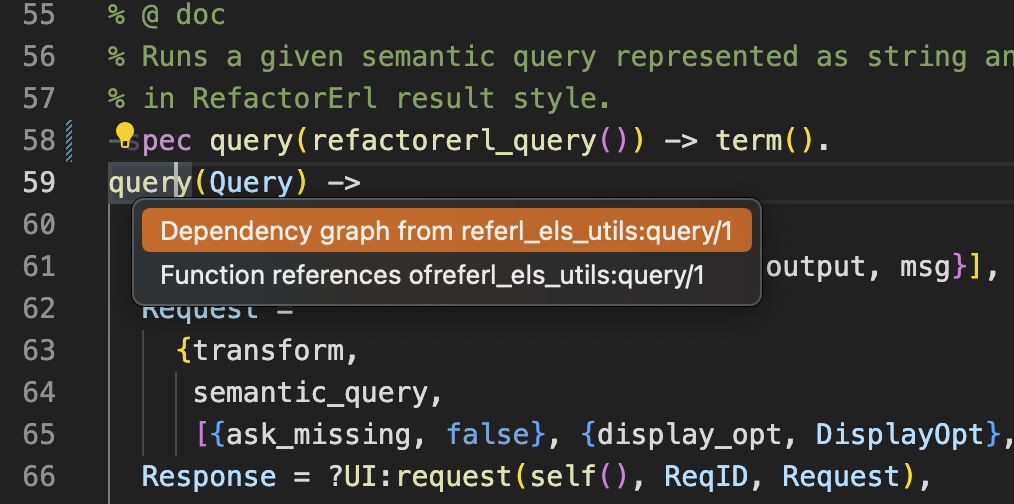
\includegraphics[width=0.7\linewidth]{images/codeact_function.png}
  \caption{Függvényhez kapcsolódó kódakciók}
  \label{fig:codeact_function}
\end{figure}

\begin{figure}[H]
  \centering
  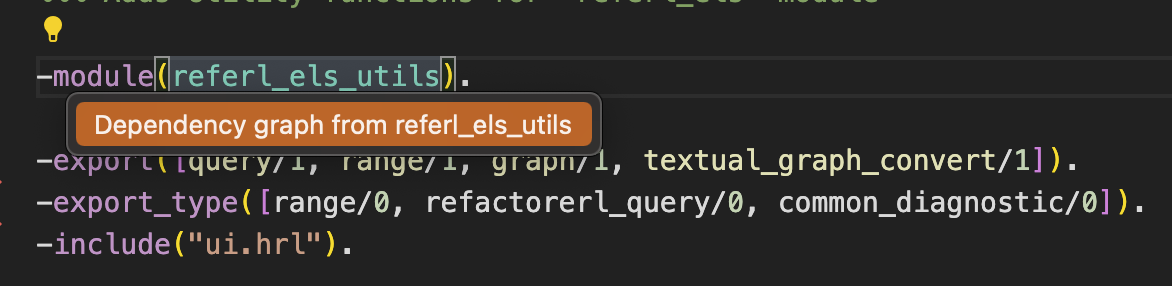
\includegraphics[width=0.7\linewidth]{images/codeact_module.png}
  \caption{Modulhoz kapcsolódó kódakciók}
  \label{fig:codeact_module}
\end{figure}

\begin{figure}[H]
  \centering
  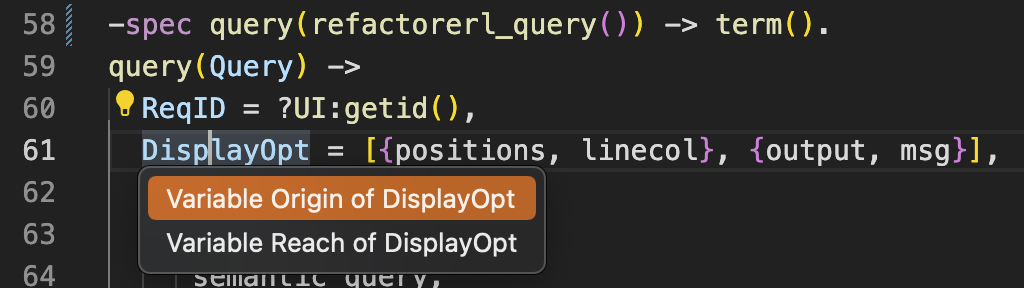
\includegraphics[width=0.7\linewidth]{images/codeact_variable.png}
  \caption{Változóhoz kapcsolódó kódakciók}
  \label{fig:codeact_variable}
\end{figure}

A kódakció elvégézéshez a kurzorral álljunk a változó, függvény vagy a modul definíció fölé és a megjelenő lámpa ikonra kattintva válasszuk ki a megfelelő opciót a helyi menüből. (lásd: \ref{fig:codeact_function}, \ref{fig:codeact_module} és \ref{fig:codeact_variable} ábrák)

\noindent \textit{Dependenc graph from Example} opció a függőségi gráfot fogja kirajzolni a megfelelő kiindulási pontból.

\noindent \textit{Variable Origin/Reach of Example} opciók rendre a változó Origin, illetve Reach értékét adják vissza.

Amikor kódakcióból indítunk beépített lekérdezést, akkor az adott fájl amiből indítjuk, hozzá lesz adva az adatbázishoz, vagy szinkronizáció el lesz végezve, de \textbf{csak arra az adott fájlra, ahonnan a parancsot kiadjuk}.

\section{Visualiser kiegészítő használata}
\subsection{Elindítása}

Az elindításhoz nincsen más teendőnk, mint az oldalsávon megjelenő RefactorErl logóra kattintani (lásd: \ref{fig:start_visualiser} ábra), továbbá a RefactorErl node-on az alábbi parancsot kiadni:

\noindent \lstinline{referl_vsc:start().} vagy \lstinline{ri:start_vsc().}

\noindent \lstinline{referl_vsc:stop().} agy \lstinline{ri:stop_vsc().} parancsokkal pedig leállíthatjuk.

\begin{figure}[H]
  \centering
  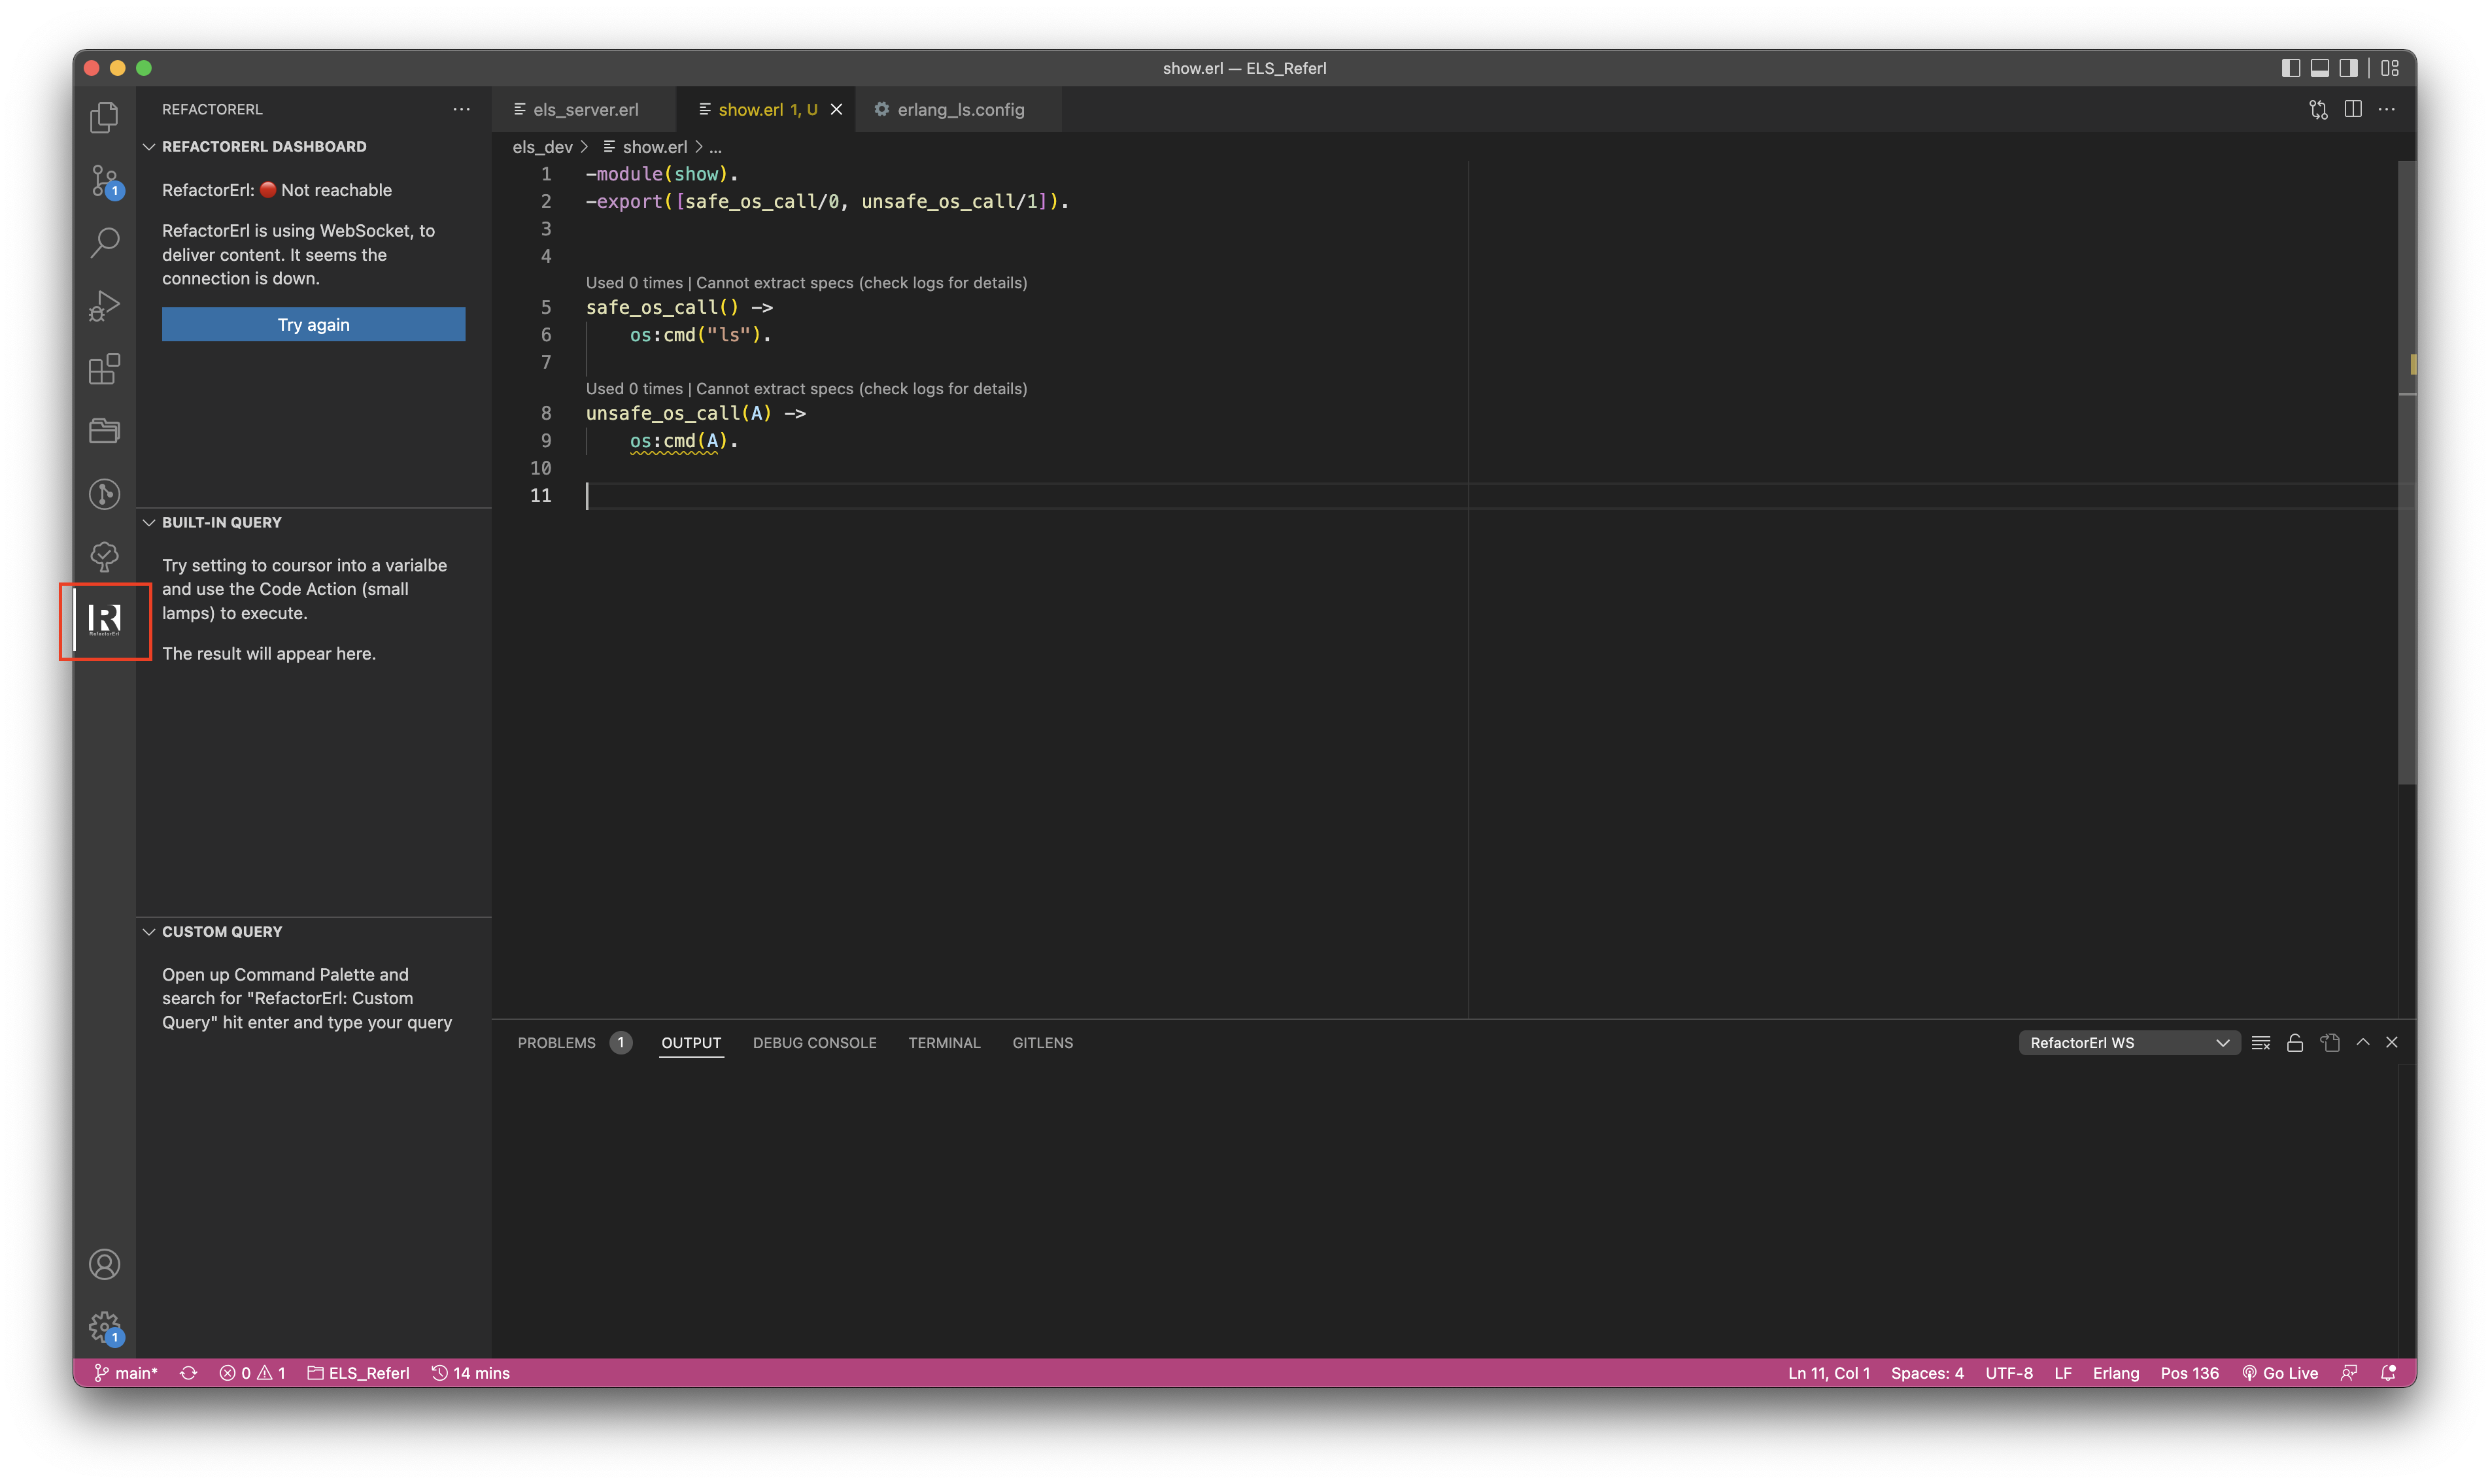
\includegraphics[width=\linewidth, clip=true, trim = 0mm 0mm 150mm 0mm]{images/start_visualiser.png}
  \caption{RefactorErl Visualiser indítása}
  \label{fig:start_visualiser}
\end{figure}


\subsection{Egyéni szemantikus lekérdezések}
A kiegészítő segítségével egyedi szemantikus lekérdezéseket is futtathatunk a RefactorErl adatbázisában tárolt fájlokon. A szemantikus lekérdezéseket az eszköz lekérdező nyelvének segítségével foglmazhatjuk meg, melyről bővebb információt a projekt wiki oldalán találhatunk \cite{referlWikiSemanticQuery}. \cite{actaelect11}

Ahhoz, hogy egy ilyen lekérdezést futtassunk az ún. \textit{Command Pallette}-et nyissuk meg, amit mac OS-en a \lstinline{CMD + SHIFT + P}, Windows-on és Linux operációs rendszeren pedig a \lstinline{CTRL + SHIFT + P} billenytűk egyidejű lenyomásával tudunk elő hozni. Itt kezdjük el gépelni a parancs nevét: \textit{Custom Query}, majd a megjelenő lehetőségek közül válasszuk ki a \textit{RefactorErl} prefixxel ellátott opciót. (lásd: \ref{fig:custom_query_palette} ábra)
\begin{figure}[H]
  \centering
  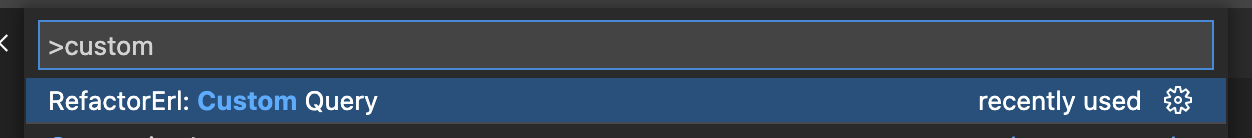
\includegraphics[width=\linewidth]{images/custom_query_palette.png}
  \caption{Custom Query megnyitása a Command Palette felületéről}
  \label{fig:custom_query_palette}
\end{figure}

Ez után a \textit{Command Palette} helyén megjelenik egy beviteli mező, ahova beírhatjuk a lekérdezést. (lásd: \ref{fig:custom_query_input} ábra)

\begin{figure}[H]
  \centering
  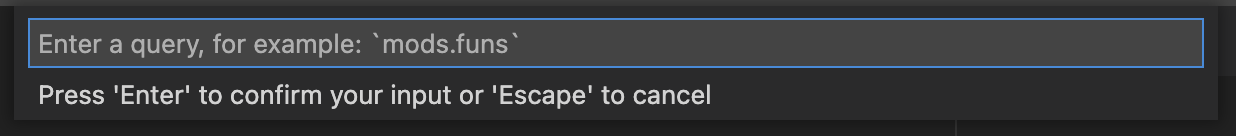
\includegraphics[width=\linewidth]{images/custom_query_input.png}
  \caption{Beviteli mező a Query számára}
  \label{fig:custom_query_input}
\end{figure}

A lekérdezést az \textit{Esc} billenytű lenyomásával megszakíthatjuk, azt \textit{Enter} segítségével pedig elküldhetjük azt. A lekérdezés állapotáról a jobb alsó sarokban kaphatunk információt. (lásd: \ref{fig:notifications} ábra)

\begin{figure}[H]
  \centering
  
\includegraphics[width=0.45\linewidth]{images/notification_done.png}
  
\includegraphics[width=0.45\linewidth]{images/notification_error.png}
  
\includegraphics[width=0.45\linewidth]{images/notification_running.png}

  \caption{Lehetséges  értesítések lekérdezés esetén}
  \label{fig:notifications}
\end{figure}

Fontos kiemleni, hogy a kódakciókkal ellentétben, az egyedi lekérdezéseknél semmiféle adatbázis szinkronizáció nem történik. Amennyiben szeretnénk egy fájlt hozzáadni, úgy a \ref{referlConfig}
fejezetben tárgyaltak szerint megtehetjük, vagy használhatjuk a bővítmény szinkronizáló funkcióját a \ref{referlDashboard} fejezetben leírtak alapján. Az egyedi lekérdezések megjelenítését a \ref{customQueryView} fejezetben fogjuk tárgyalni.



\subsection{Függőségi gráf rajzolása} \label{sectionDepGraph}

Függőségi gráfot tudunk rajzolni kódakciók segítésével, illetve a \textit{RefactorErl: Dependencies} nézet segítségével, itt az utóbbit fogjuk megtekinteni.

A nézet előhozásához a \textit{Command Palette}-n írjuk be, hogy: \textit{Dependenc Graph Visualiser}. Majd meg is jelenik a nézet. (lásd \ref{fig:depGraphView} ábra)

\begin{figure}[H]
  \centering
  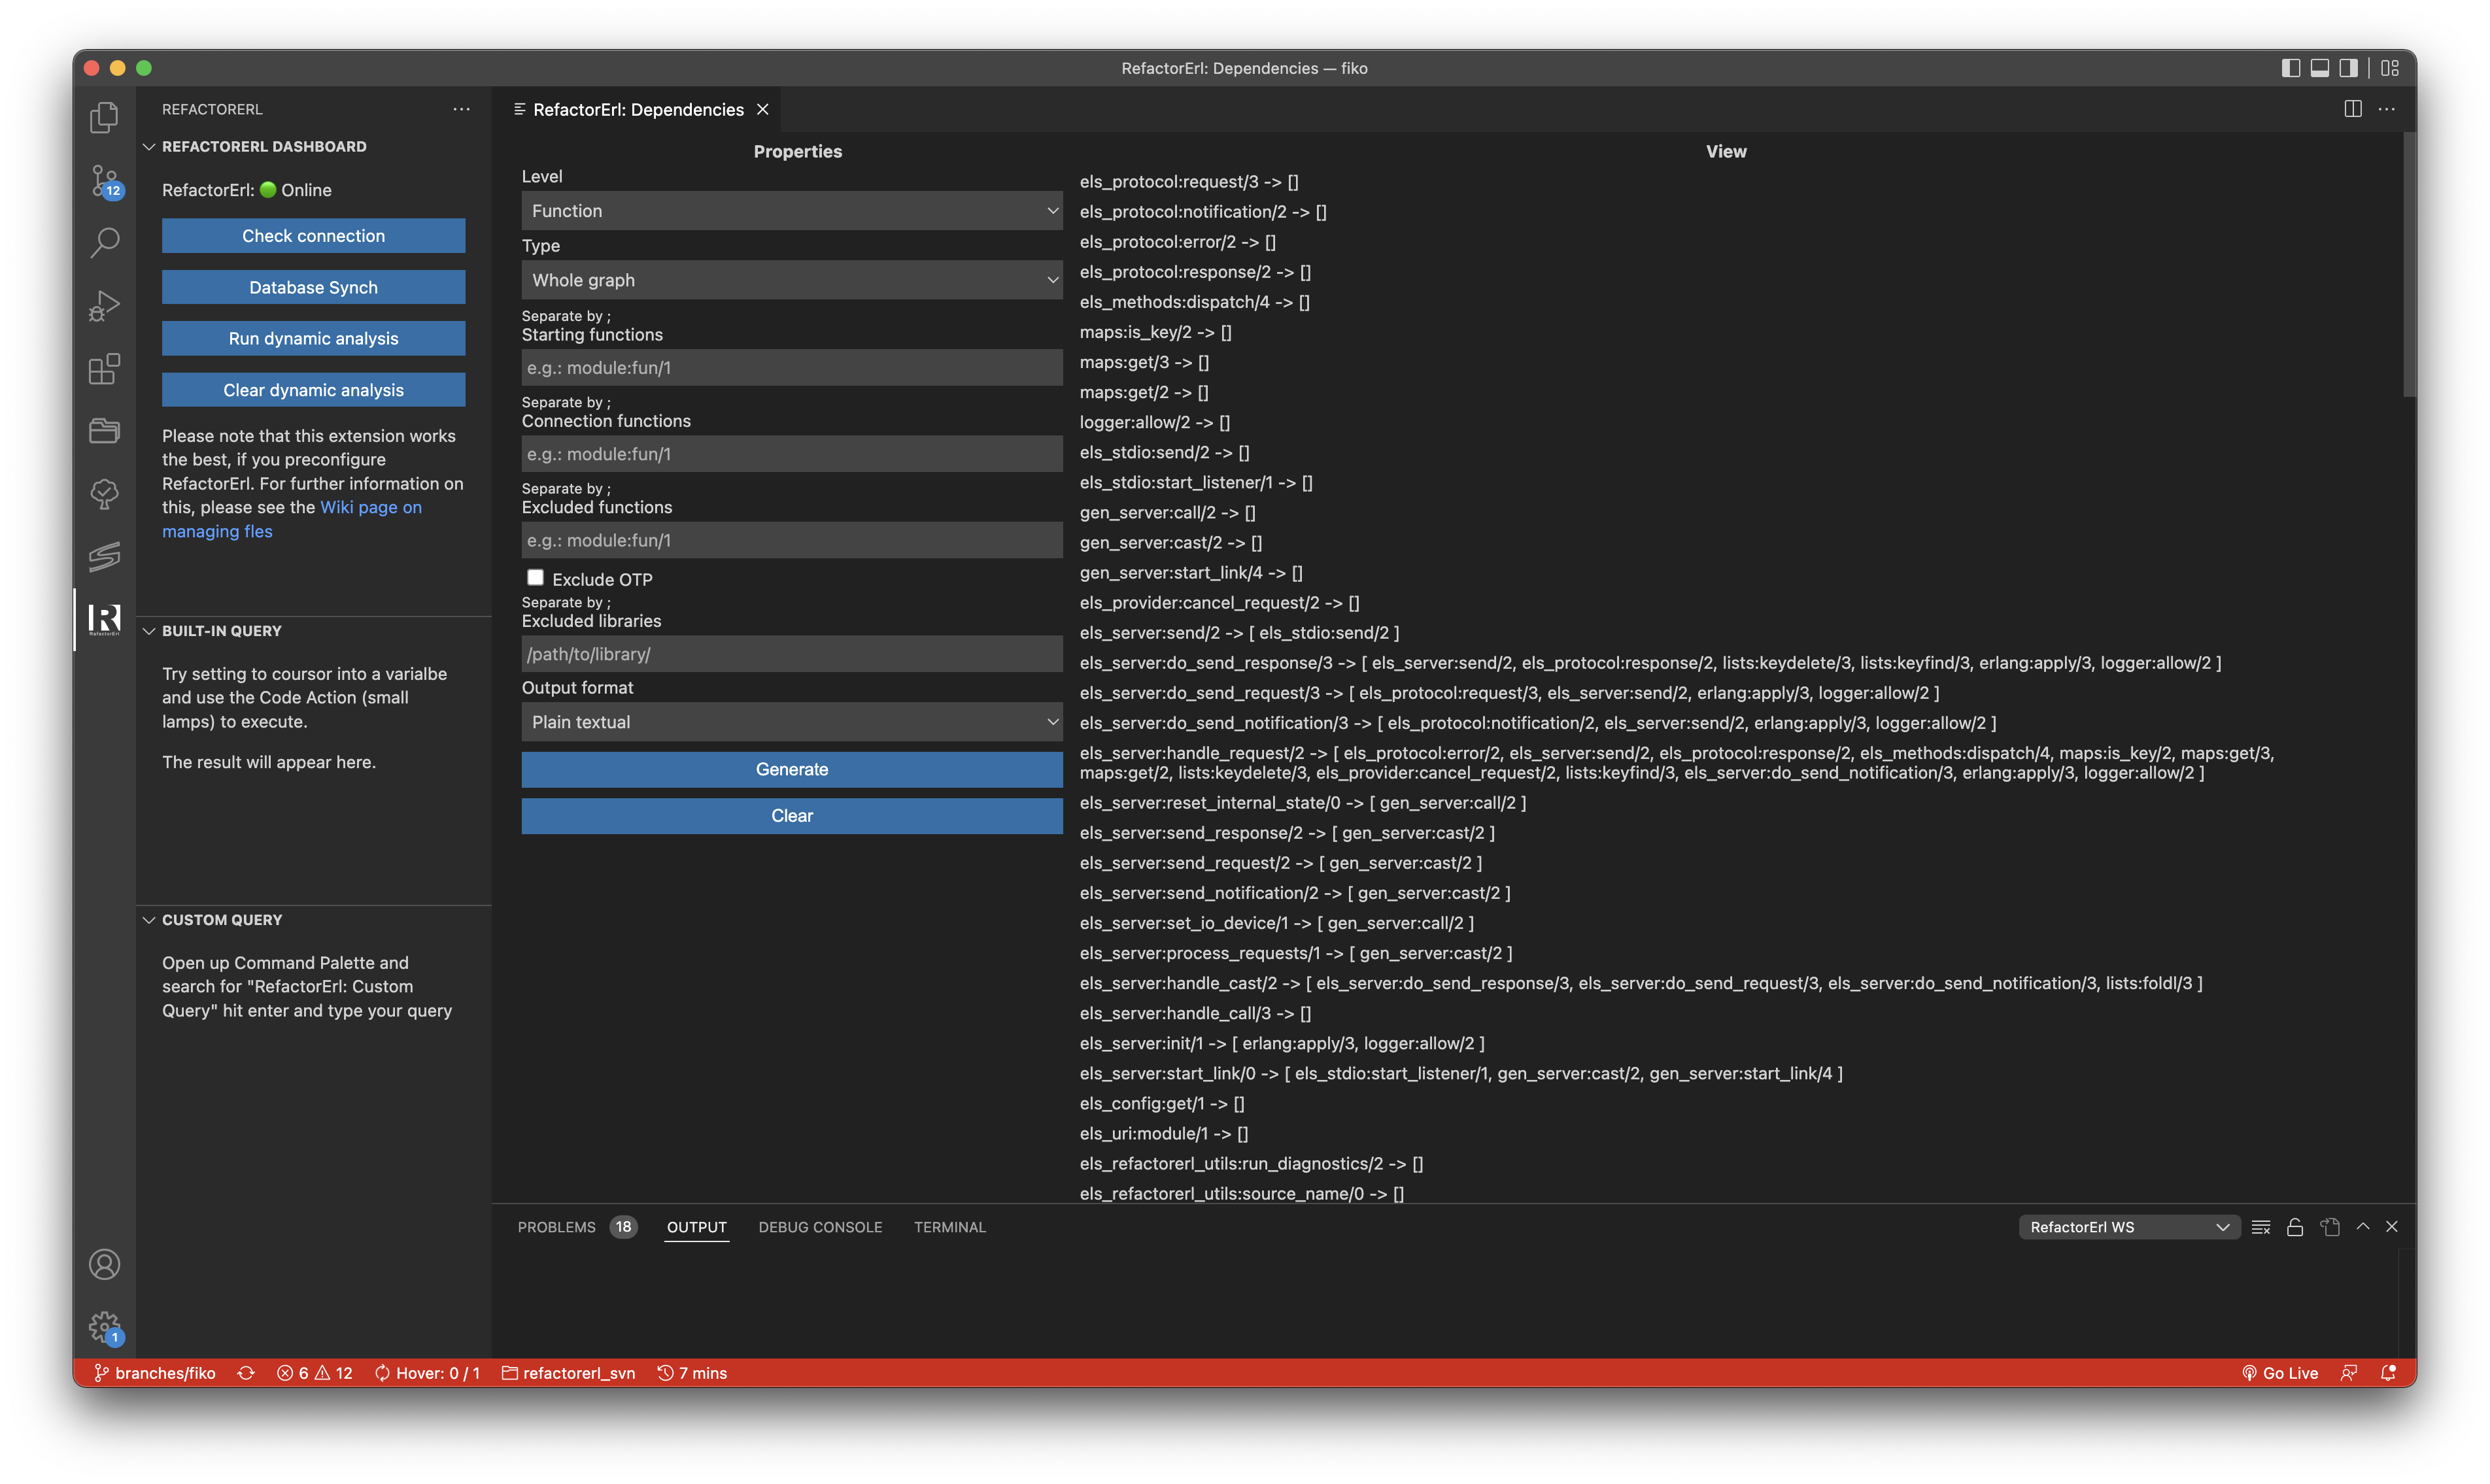
\includegraphics[width=\linewidth, clip=true, trim = 0mm 0mm 200mm 0mm]{images/dependency.png}
  \caption{Függöségi gráf nézete a bővítményben}
  \label{fig:depGraphView}
\end{figure}

Ammenyiben a nézetből szeretnénk generálni a gráfot, úgy az alábbi lehetősgek állnak rendelkezésre az oldalsó részen: (bővebben a Wiki oldalon olvashatunk a szűrési opciókról (Filtering options) \cite{referlWikiDependency})

\begin{itemize}
    \item \textbf{Level}: típusa, lehet \textit{Function} (függvény) vagy \textit{Module} (modul). Azt tudjuk meghatározni, hogy milyen szinten legyen a gráf generálva
     \item \textbf{Type}: típusa, lehet \textit{Whole graph} (teljes gráf) vagy \textit{Cyclic sub-graph} (ciklikus részgráf).
     \item \textbf{Starting functions/modules}: megadhatjuk, hogy mely függvények vagy modulok legyenek a kezdő pontok. Ha többet szeretnénk megadni, akkor pontos vesszővel válasszuk el.
     \item \textbf{Connection functions/modules}: megadhatjuk, hogy mely függvények vagy modulok legyenek a kapcsolódási pontok. Ha többet szeretnénk megadni, akkor pontos vesszővel válasszuk el.
     \item \textbf{Excluded functions/modules}: megadhatjuk, hogy mely függvények vagy modulok legyenek kizárva. Ha többet szeretnénk megadni, akkor pontos vesszővel válasszuk el.
     \item \textbf{Excluded OTP}: Amennyiben ezt bejelöljük, úgy az OTP függvényei, moduljai ki lesznek zárva a gráfból.
     \item \textbf{Excluded libraries}: megadhatjuk, hogy mely könyvtárak legyenek kizárva. Ha többet szeretnénk megadni, akkor pontos vesszővel válasszuk el.
     \item \textbf{Output format}: kimeneti formátum, lehet \textit{Plain textual} (szöveges reprezentáció) vagy \textit{SVG} 
\end{itemize}

Végül rendelkezésre áll egy \textit{Generate} és egy \textit{Clear} feliratú gomb. A feladatuk rendere a gráf generálása, létrehozása illetve a generált gráf törlése. Szöveges reprezentáció esetén az eredmény jobb oldalt a nagyobb munkaterületen jelenik meg. SVG opció esetén egy új fülön fog megjelenni, s a munkaterületen egy hivatkozás, gomb fog megjelenni. (lásd: \ref{fig:depGraphSVG} ábra)

\begin{figure}[H]
  \centering
  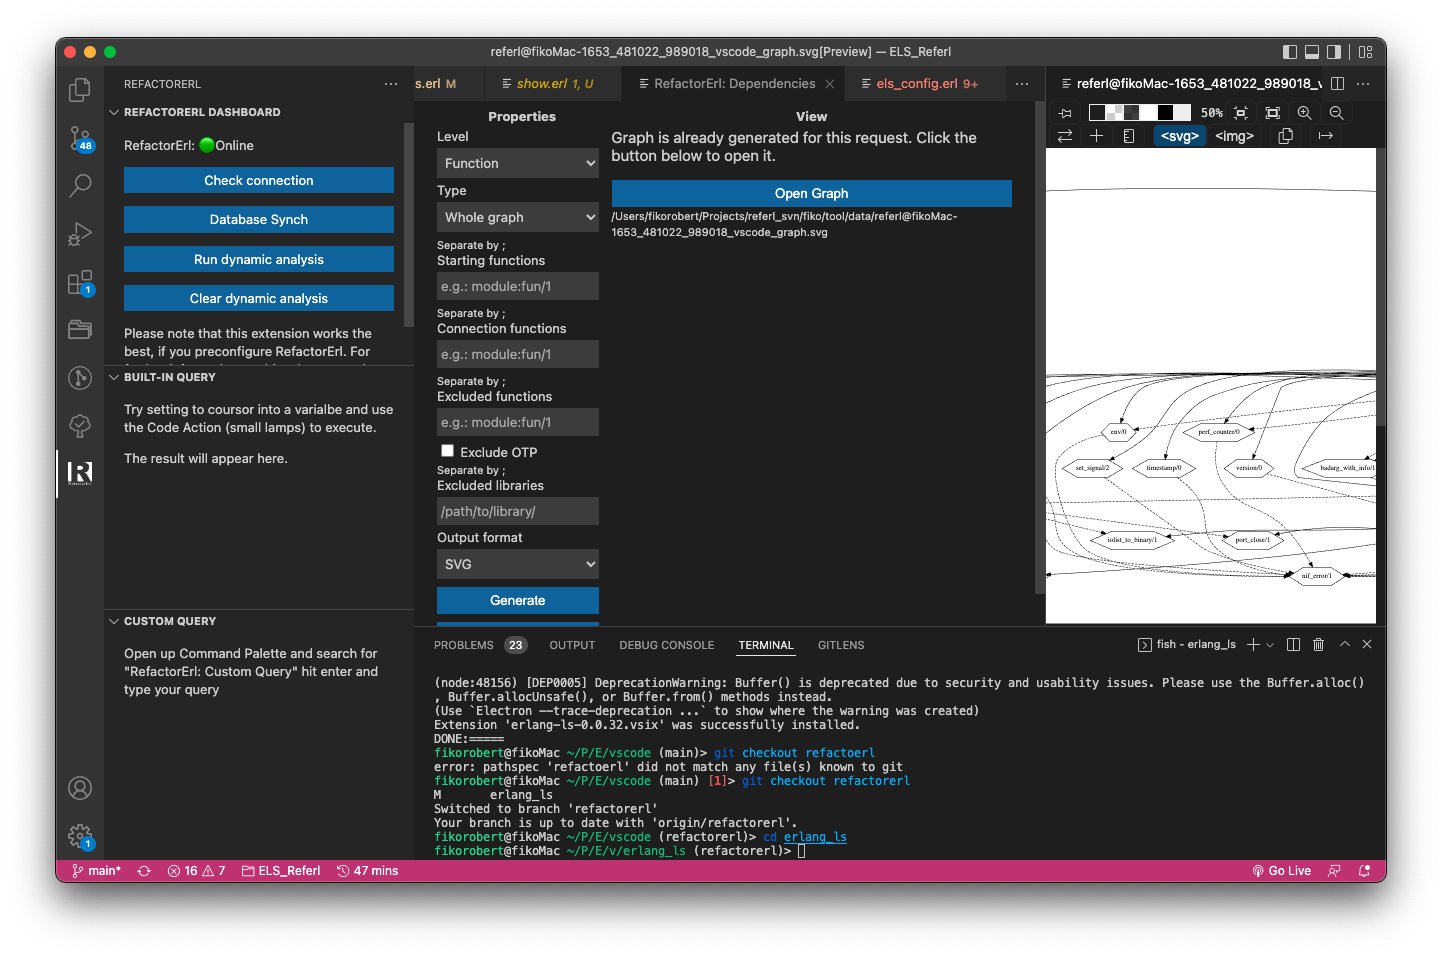
\includegraphics[width=\linewidth]{images/svg_graph.png}
  \caption{Függöségi gráf SVG opcióval}
  \label{fig:depGraphSVG}
\end{figure}

\newpage

\subsection{Az oldalsáv funkcionalitásai}

\begin{wrapfigure}[23]{L}{0.5\textwidth}
\centering
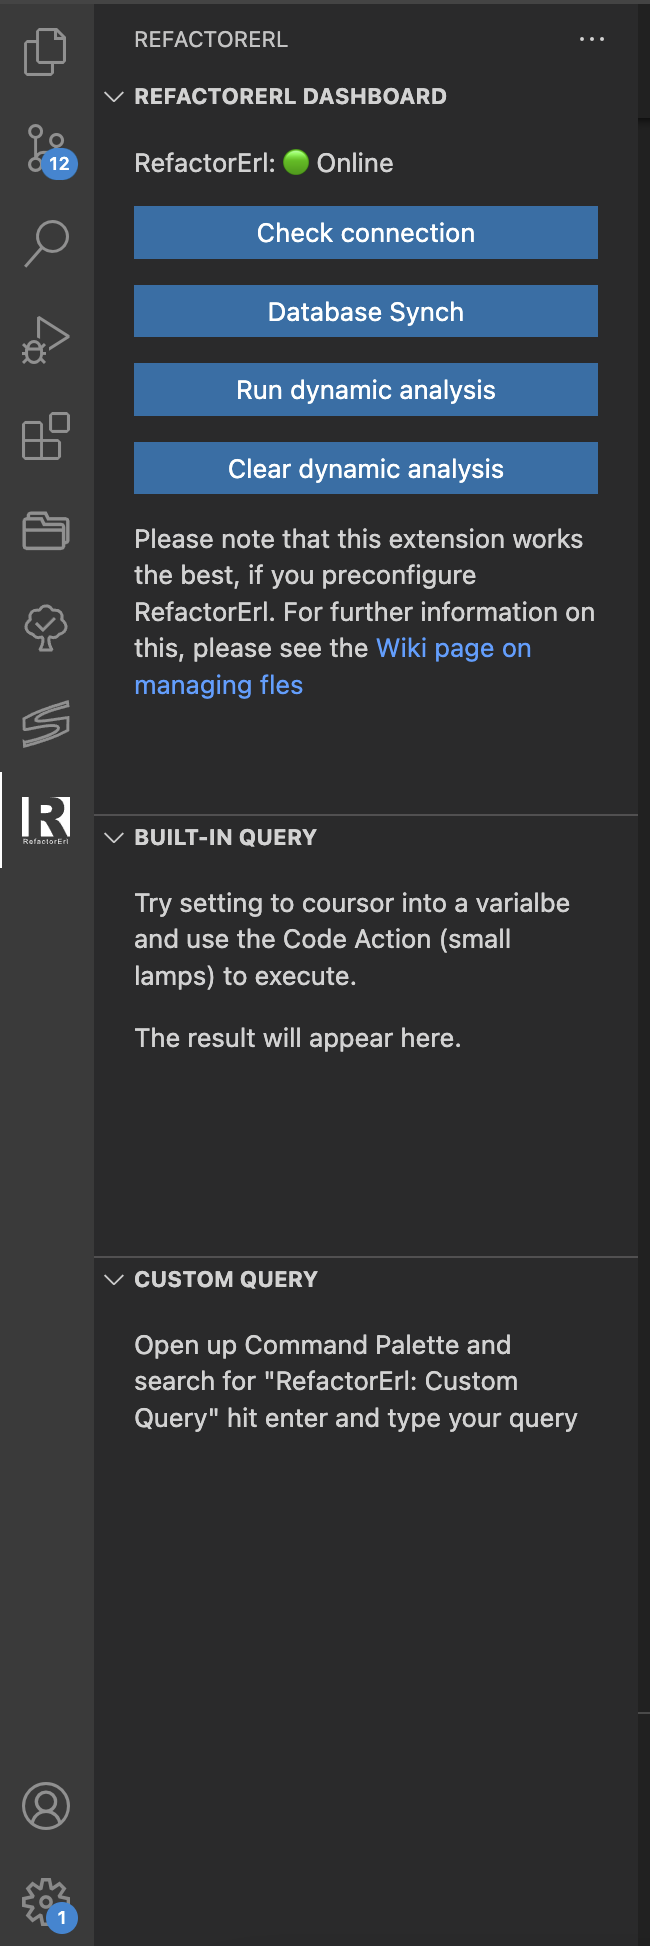
\includegraphics[width=0.45\textwidth]{images/sidebar_active.png}
\caption{\label{fig:sidebar_active} Oldalsáv funkcionalításai}
\end{wrapfigure}

Az \ref{fig:sidebar_active} ábra alapján tekintsük át az odalsávon elérhető funkcionalitásokat. 

\textit{Megjegyzés: A \ref{fig:sidebar_active} ábrán látott sorrendtől a felhasználó sorrendje eltérhet, hiszen ezen panelek szabadon átrendezhetőek. A bemutatásnál a \ref{fig:sidebar_active} ábrán látható sorrendet követjük.}

Fő panelek áttekintése:

\begin{itemize}
    \item \textbf{RefactorErl Dashboard\footnote{Vezérlőpult}} Itt láthatjuk a RefactorErl node állapotát, illetve néhány vezérlő gomb segítségével ellenőrizhetjük a kapcsolatot, szinkronizálhatjuk az adatbázist, illetve lefuttathatjuk  a dinamikus elemzést vagy éppen törölhetjük annak erdeményét.
    \item \textbf{Built-In Query} Ezen panelen fognak megjelenni a beépített lekérdezések eredményei, mint például: \textit{Variable Reach} \textit{Variable Origin}, vagyis változó lehetséges értékei és dinamikus függvény hivatkozások eredményei.
    \item \textbf{Custom Query} Ebben a nézetben jelennek a meg a \textit{Command Palette}-n beírt egyedi lekérdezések eredményei.
\end{itemize}

\newpage

\subsubsection{RefactorErl Dashboard} \label{referlDashboard}

\noindent \textbf{Kapcsolat állapota}

Az első információ amit a vezérlőpult jelez nekünk, a kapcsolat állapota. Ennek két állapota lehet:

\begin{itemize}
    \item Zöld jelzővel, \textit{Online}, vagyis elérhető
    \item Piros jelzővel, \textit{Not reachable}, vagyis nem elérhető
\end{itemize}

Az elérhető esetben a WebSocket alapú kapcsolat teljes mértékben létrejött és a bővítmény használható, az utóbbi esetben sajnos ez nem mondható el. Azt fontos kiemeleni, hogy ha kiegészítő számára nem elérhető a RefactorErl node, az nem azt jelenti, hogy a teljes eszköz nem fut vagy nem működik. Erről további információt a \ref{not_reachable_node} részben olvashatunk.

\vspace{5mm}
\noindent \textbf{Kapcsolat ellenőrzése}

A \textit{Check connection} feliratú gomb megnyomásával tudjuk ellenőrizni a kapcsolat állapotát. Az alábbi eredményekkel zárulhat ez a művelet:

\begin{itemize}
    \item \textbf{Sikeres kapcsolat.} Ebben az esetben a \textit{Connected to RefactorErl via WS} üzenet jelenik meg a jobb alsó sarkoban. Ez esetben a kapcsolat az eszköz és a bővítmény között WebSocketen keresztül ki van építve.
    \item \textbf{Nem lehet csatlakozni.} Ebben az esetben a \textit{Cannot connect to RefactorErl via WS} üzenetet kapjuk jobb alul. Ebben az esetben a kapcsolat kiépítése közben hiba lépett fel.
\end{itemize}

\vspace{5mm}
\noindent \textbf{Adatbázis szinkronizálása} 
A \textit{Database Synch} feliratú gombra kattintva a már betöltött fájlok frissítését tudjuk kérvényezni, amennyiben azokban történt változás. A folyamat állapotáról a jobb alsó sarokban a rendszer tájékoztat.

\vspace{5mm}
\noindent \textbf{Dinamikus függvényhívás elemzés elvégézése}
A \textit{Run dynamic analysis} címkéjű gomb segítségével a betöltött állományokon a dinamikus elemzést végezhetünk el. A folyamat állapotáról a jobb alsó sarokban a rendszer tájékoztat.

\vspace{5mm}
\noindent \textbf{Dinamikus függvényhívás elemzés eredményének törlése}
A \textit{Clear dynamic analysis} gomb megnyomásával a már elvégzett dinamikus elemzést törölhetjük. Ez akkor lehet fontos, amikor az adatbáziban változás lépett fel. A folyamat állapotáról a jobb alsó sarokban a rendszer tájékoztat.


\subsubsection{Built-In Query megjelenítője} \label{sectionVariable}

A második panelen a beépített lekérdezések megjelenítését találhatjuk. Amennyiban az Erlang LS-ből kódakciók segítségével indítjuk a lekérdezést, abban az esetben ebben a középső\footnote{A panelek tetszőlgesen átrendezhetőek, de az ábrán és alapértelmezetten középső} panelben jelenik meg az eredény, egy \textit{fa szerkezetű listában}. Ha a listában egy értékere kattintunk, akkor bővítmény az adott eredményre visz, amennyiben van pozíció adat hozzá a RefactorErl adatbázisban.

Itt jelennek meg az alábbi beépített lekérdezések
\begin{itemize}
    \item Variable Origin
    \item Variable Reach
    \item Dinamikus függvény hívások
\end{itemize}

\begin{figure}[H]
  \centering
  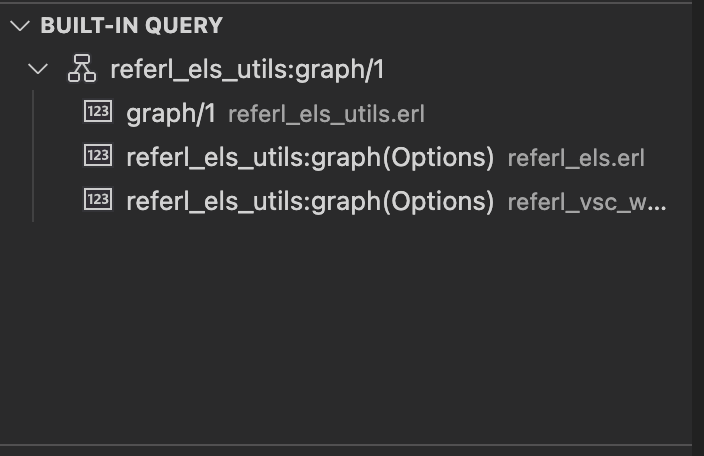
\includegraphics[width=0.5\linewidth]{images/builtin_query.png}
  \caption{Dinamikus függvény hívások a Built-In Query megjelenítőben}
  \label{fig:bultin_query_view}
\end{figure}

\subsubsection{Custom Query megjelenítője} \label{customQueryView}

Az egyedi lekérdetések megjelenítője nagyon hasonló a beépítettéhez. Itt is egy \textit{fa szerkezetű listában} jelennek meg az adatok, és kattintásra ugyaúgy az eredményhez vihetnek.
(lásd: \ref{fig:custom_query_view} ábra)

\begin{figure}[H]
  \centering
  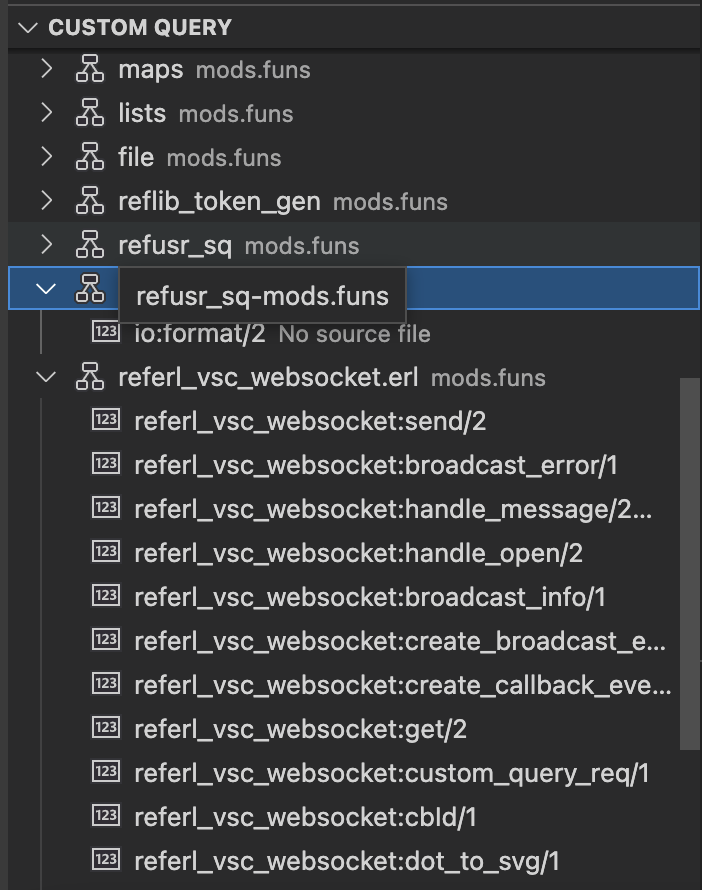
\includegraphics[width=0.4\linewidth]{images/custom_query.png}
  \caption{Egyedi \lstinline{mods.funs} lekérdezés a Custom Query megjelenítőben}
  \label{fig:custom_query_view}
\end{figure}

Egyedi lekérdezések esetében gyakrabban belefuthatunk a pozíció nélküli eredménybe. (lásd: \ref{fig:nopos_res} ábra) Az ilyen eredmény mellett látjuk a \textit{No source file} alcímet, ami ezt jelzi nekünk. Erre való kattintás esetén hiba üzenet jelzi, hogy nem tudunk semmilyen pozícióra menni. Ez olyankor fordulhat elő, amikor meghívunk egy olyan függvényt, ami ugyan egy másik modulban jelene van, de annak a modulnak a forrása nincsen betöltve a RefactorErl-be, így nem tudunk hozzá lokációt adni.

Ammenyiben a pozíció adat rendelkezésre áll, úgy a megfelelő helyre visz a bővítmény. (lásd: \ref{fig:code_highligh} ábra)

\begin{figure}[H]
  \centering
  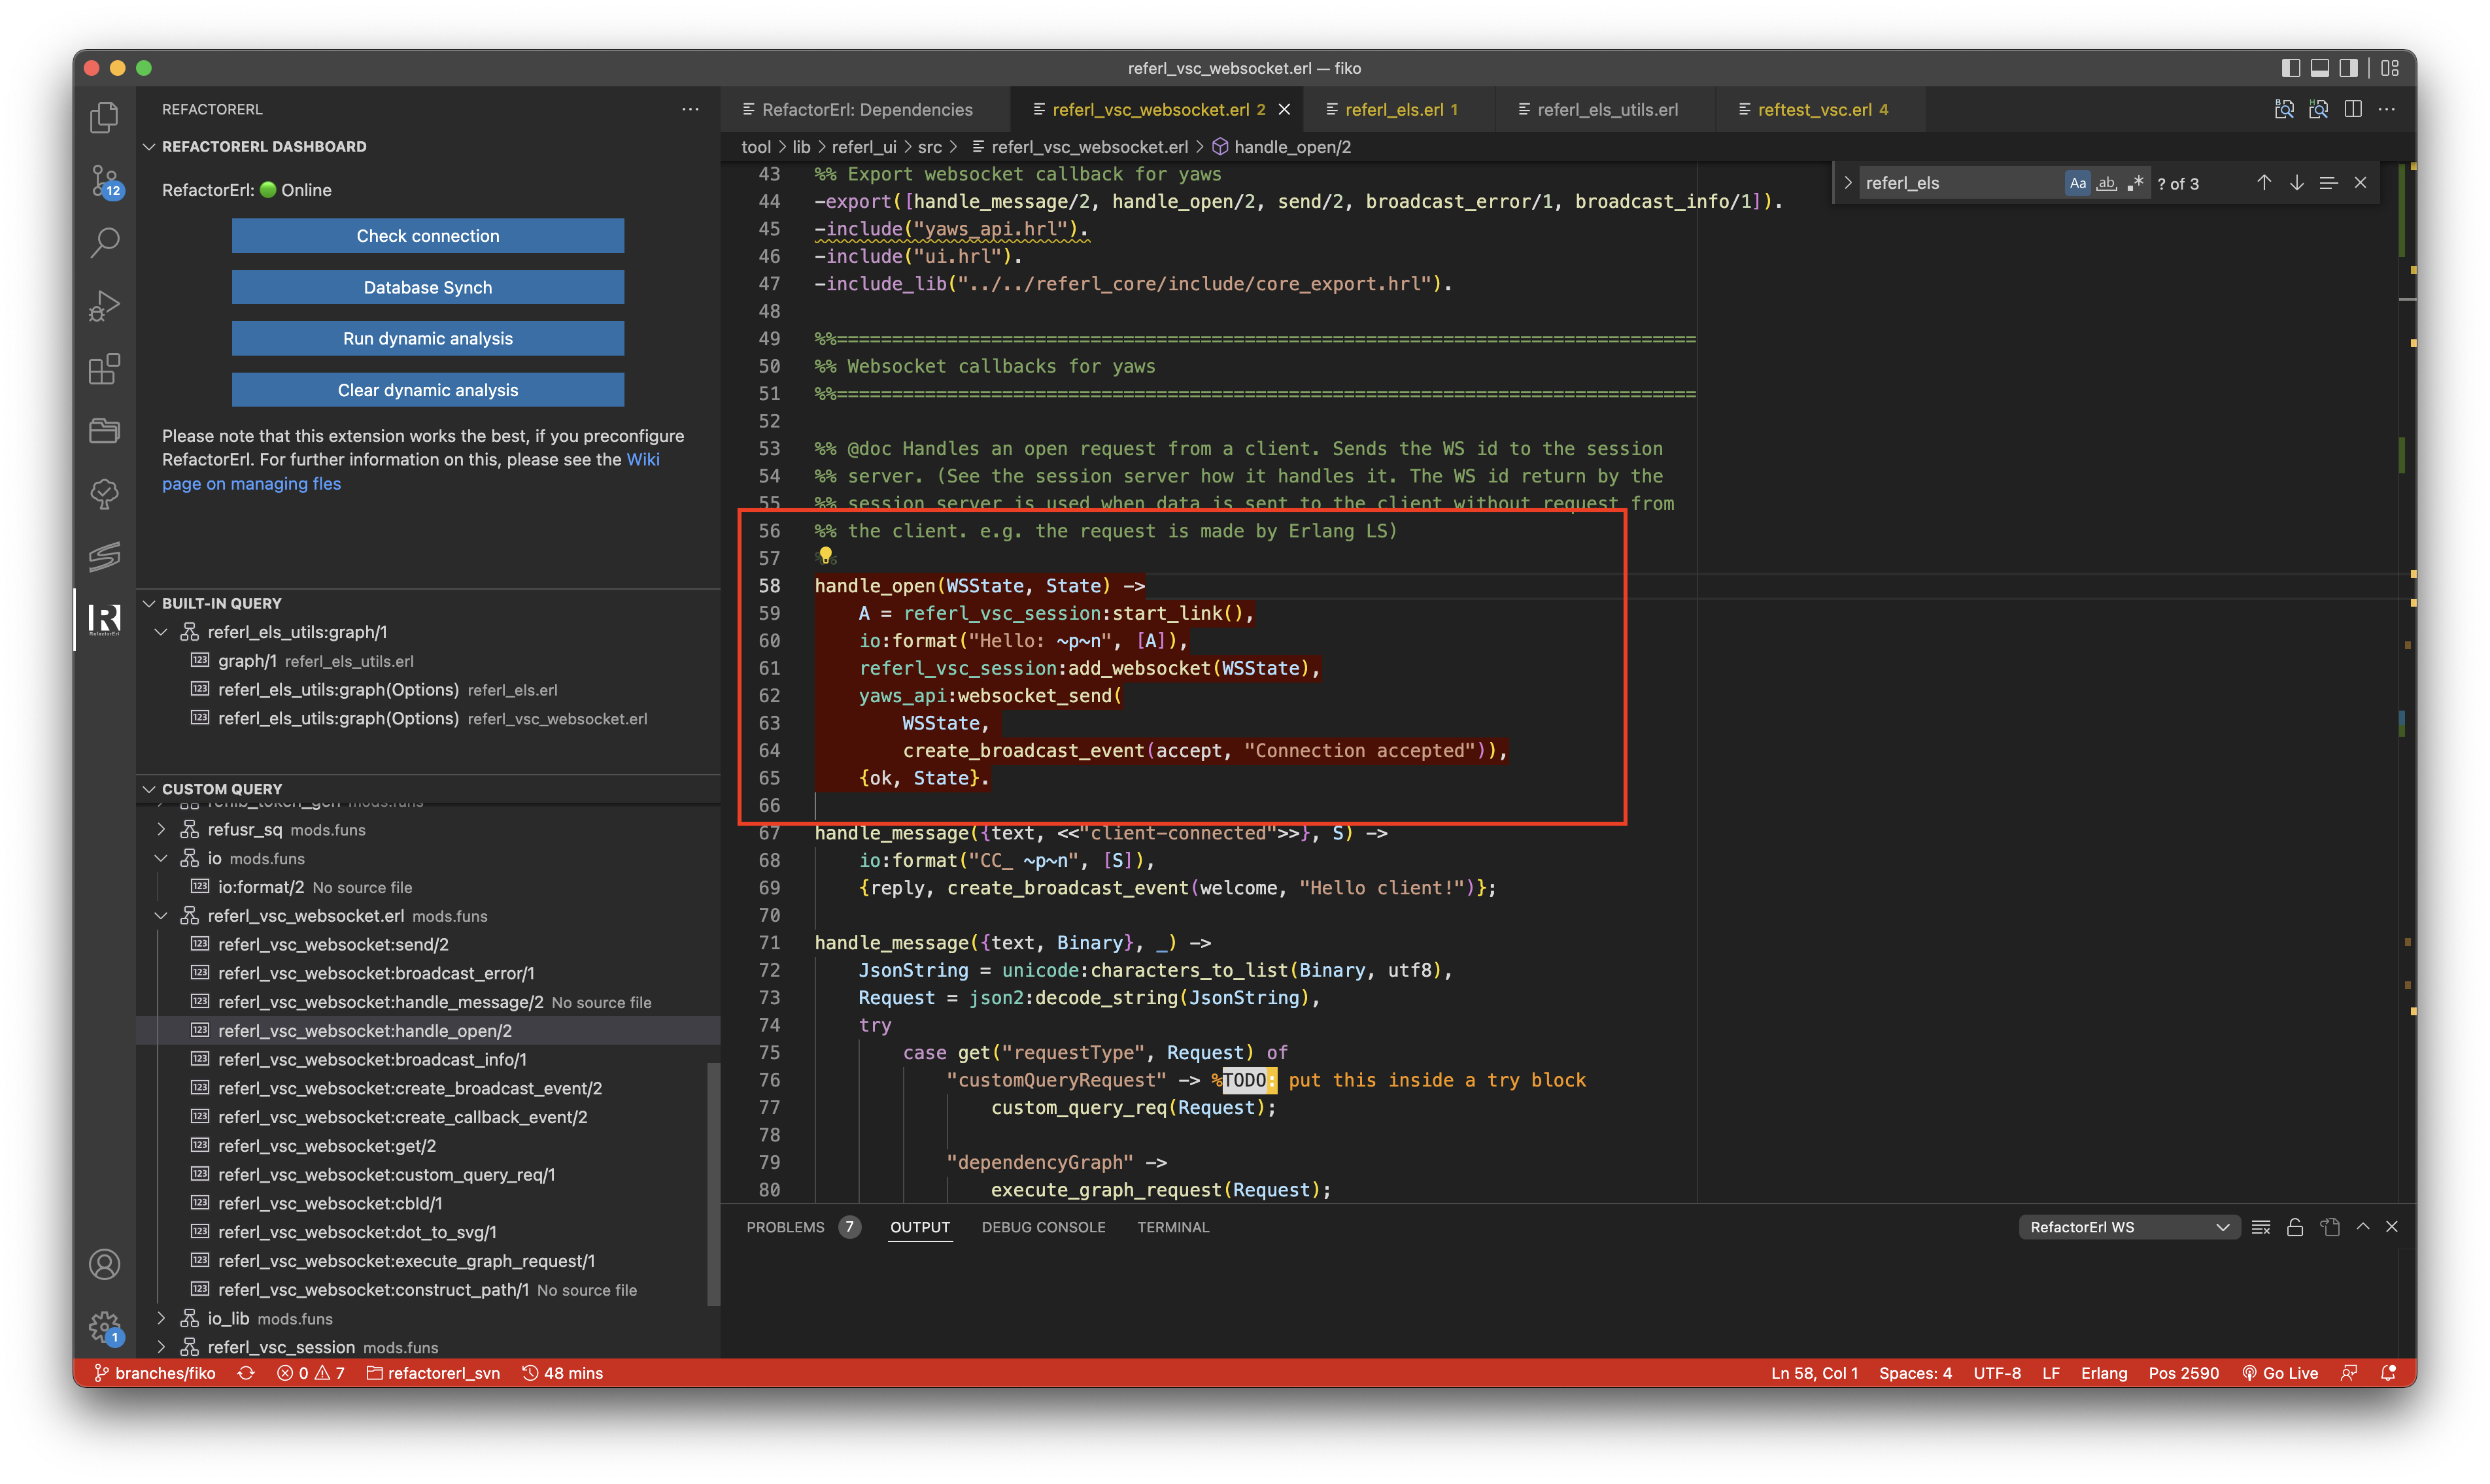
\includegraphics[width=\linewidth]{images/code_highlight.png}
  \caption{Pozícióval rendelkező eredmény kódkiemelése a szerkesztőben}
  \label{fig:code_highligh}
\end{figure}

\begin{figure}[H]
  \centering
  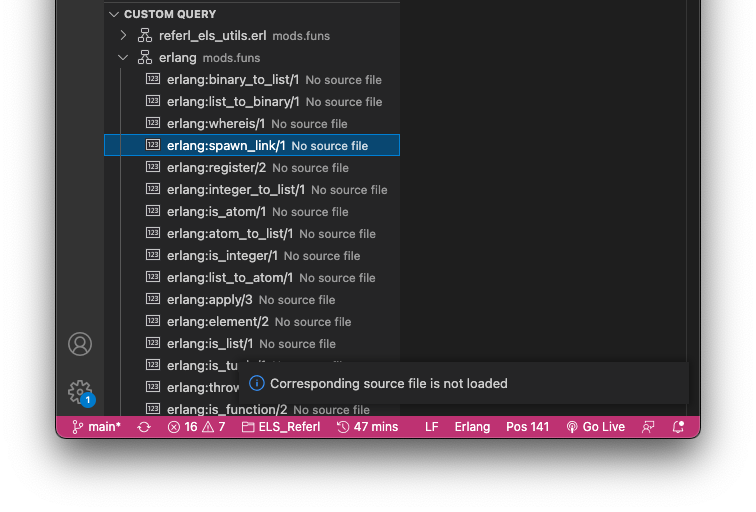
\includegraphics[width=\linewidth]{images/nopos.png}
  \caption{Pozíció nélküli eredmény megjelenítése}
  \label{fig:nopos_res}
\end{figure}



\section{Probléma elhárítás}
\subsection{Ha a node nem elérhető a bővítmény szerint} \label{not_reachable_node}

Ez esetben győződjünk meg arról, hogy az Erlang node, amin a RefactorErl fut, az elérhető-e. Ehhez használhatjuk a \lstinline{epmd -names} parancsot, ami listázza a futó Erlang node-okat.
Valami hasonló kimenetet kell várnunk, mint a \ref{epmdSample} forrásban, amennyiben fut a RefactorErl. Itt a node nevét kell látnunk.

\lstset{caption=Erlang Port Mapper Deamon (epmd) példa kimenete, label=src:sh}  \label{epmdSample}
\begin{lstlisting}[language={sh}] 
fikorobert@fikoMac ~> epmd -names
epmd: up and running on port 4369 with data:
name erlang_ls_fiko_121933337 at port 55854
name referl at port 55652
...
\end{lstlisting}


Továbbá még használható a \lstinline{net_adm:ping/1} \footnote{\url{https://www.erlang.org/doc/man/net_adm.html##ping-1}} függvénye is, ahol a paraméterül adjuk meg egy nevesített Erlang node shelljében, az adott node nevét és \lstinline{pong}-al tér vissza, akkor rendben van, ha \lstinline{pang}-al akkor nincs rendben.

Továbbá győződjünk meg arról, hogy a VSC applikáció fut-e. Az elindításhoz használjuk a \lstinline{referl_vsc:start().}, leállításhoz, pedig a \lstinline{referl_vsc:stop().} hívásokat. Ezek után a \textit{Try again} gombbal próbáljunk újra csatlakozni.
